\section{Results}

\subsection{Global Totals Are Narrow and Domain-Skewed}

Table~\ref{tab:model-summary} gives the exact official totals for the comparable
open-8 cohort. The raw totals are already modest: the top three models each
reach only $5/54$ official \resultmetric success, while three models remain at
$0/54$ on both official fields. Figure~\ref{fig:overview} adds the broader
distributional picture. Official success is not spread evenly across the
benchmark. In the open-8 cohort, office-document families contribute $10/72$
\resultmetric successes, security contributes $7/72$, web contributes $2/48$,
and speech contributes $2/64$. Physiological signals show two
\processmetric-true traces but zero \resultmetric successes. Image and video are
complete zeros.

\begin{table}[t]
\caption{Official GitTaskBench summary on the comparable local cohort.}
\label{tab:model-summary}
\centering
\small
\begin{tabular}{lcc}
\toprule
Model & Process & Result \\
\midrule
Qwen2.5-14B & 9 & 5 \\
Qwen3-32B & 8 & 5 \\
Qwen2.5-32B & 7 & 5 \\
Qwen3-14B & 6 & 4 \\
Mistral-Small-24B & 2 & 2 \\
DeepSeek-R1-D8B & 0 & 0 \\
Mistral-7B & 0 & 0 \\
Qwen2.5-7B & 0 & 0 \\
\bottomrule
\end{tabular}
\end{table}


\begin{figure*}[t]
    \centering
    \begin{subfigure}[t]{0.58\textwidth}
        \centering
        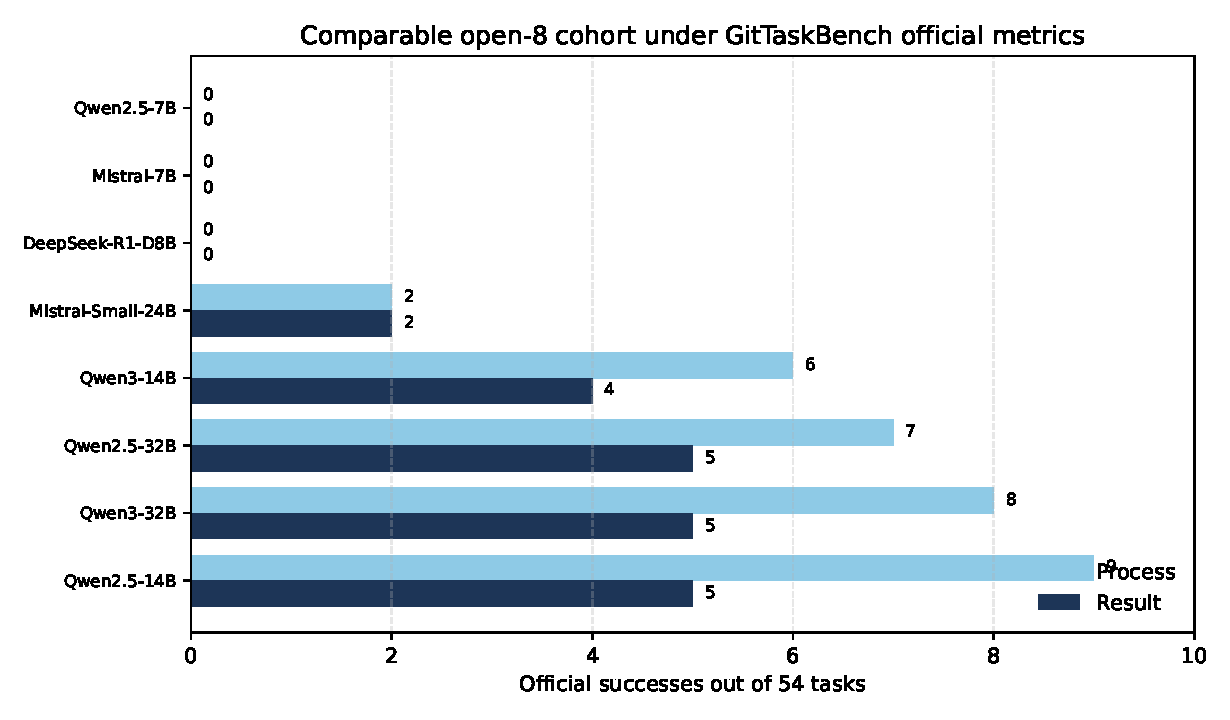
\includegraphics[width=\textwidth]{figures/figure_model_summary.pdf}
        \caption{Comparable open-8 official totals.}
    \end{subfigure}
    \hfill
    \begin{subfigure}[t]{0.38\textwidth}
        \centering
        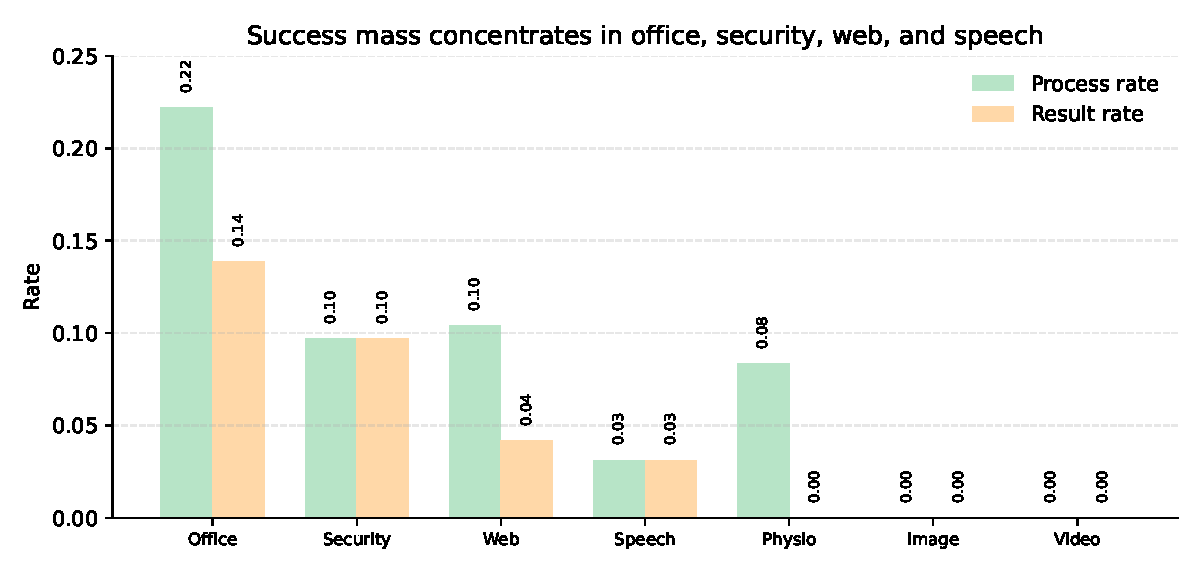
\includegraphics[width=\textwidth]{figures/figure_domain_summary.pdf}
        \caption{Paper-side rates aggregated from official outputs.}
    \end{subfigure}
    \caption{Global official scores hide a strongly skewed success distribution. The benchmark's observed success mass is concentrated in office, security, web, and speech families, while image and video are complete zeros in the open-8 local cohort.}
    \label{fig:overview}
\end{figure*}

This distribution matters because a single global score can suggest a smooth
ordering that the domain slices do not support. In our cohort, different
families occupy different parts of the official \processmetric/\resultmetric
space, and some families currently produce no observed official success at all.

\subsection{Tied Headline Scores Hide Family Specialization}

The three headline leaders in the open-8 cohort tie at $5/54$ official
\resultmetric success, but the tied total is misleading. \texttt{Qwen2.5-14B}
reaches official success in \texttt{Eparse}, \texttt{PDFPlumber}, and
\texttt{Faker}. \texttt{Qwen2.5-32B} keeps those families and adds
\texttt{SpeechBrain}. \texttt{Qwen3-32B} swaps \texttt{Eparse} for
\texttt{Trafilatura}. Figure~\ref{fig:task-heatmap} makes this visible at task
level. \texttt{Eparse\_02}, \texttt{Faker\_03}, and
\texttt{PDFPlumber\_03} are repeatable successes across multiple models, but
other wins are singleton or near-singleton events such as
\texttt{Trafilatura\_01} for \texttt{Qwen3-32B} and \texttt{Trafilatura\_03}
for \texttt{Mistral-Small-24B}.

\begin{figure}[t]
    \centering
    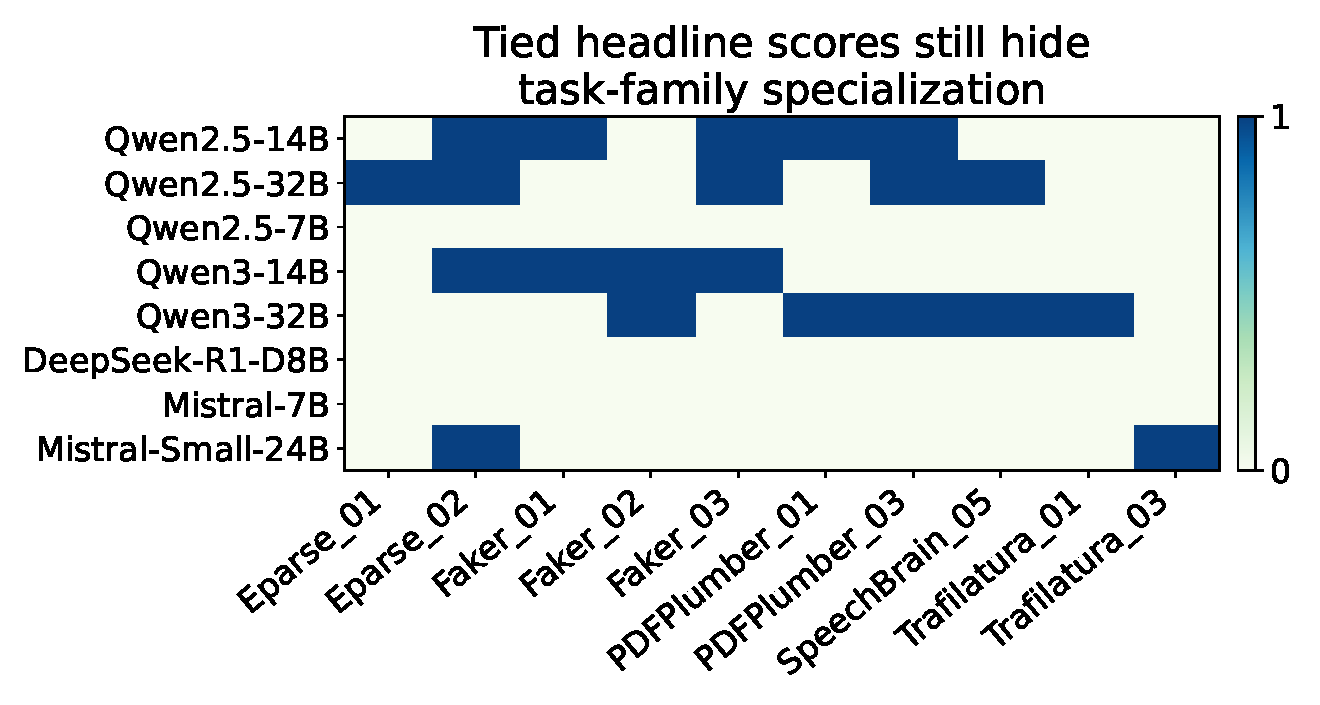
\includegraphics[width=\columnwidth]{figures/figure_task_heatmap.pdf}
    \caption{Official \resultmetric task heatmap for all tasks with at least one observed success in the open-8 cohort. Several models tie globally, but they do not win on the same task set.}
    \label{fig:task-heatmap}
\end{figure}

This is the paper's clearest measurement point. A single global success rate can
hide material specialization even before we look at trajectories, prompts, or
manual annotations. If the reporting goal is to understand what a repo-grounded
agent can actually do, the family slice matters.

\subsection{The Local Evidence Already Extends Beyond Qwen}

The open-8 comparable cohort contains only one non-Qwen model with non-zero
official \resultmetric success: \texttt{Mistral-Small-24B}
achieves $2/54$. Its wins are \texttt{Eparse\_02} and
\texttt{Trafilatura\_03}. That is enough to prevent the main observation from
reducing to a purely within-Qwen comparison, although same-task non-Qwen
coverage remains limited. The shared-task \texttt{Trafilatura} slice extends
the point further. Table~\ref{tab:shared-trafilatura} shows that
\texttt{gpt-5.2} and \texttt{Gemini-2.5-Pro} both achieve official
\processmetric$=$1, \resultmetric$=$1 on \texttt{Trafilatura\_02}. Meanwhile,
\texttt{Qwen3-32B} is the only model in the local roster that reaches official
success on \texttt{Trafilatura\_01}.

\begin{table}[t]
\caption{Latest shared-task official outcomes across all locally available models. Each cell reports Process/Result.}
\label{tab:shared-trafilatura}
\centering
\small
\begin{tabular}{lcc}
\toprule
Model & T01 & T02 \\
\midrule
Qwen2.5-14B & 0/0 & 0/0 \\
Qwen2.5-32B & 0/0 & 0/0 \\
Qwen2.5-7B & 0/0 & 0/0 \\
Qwen3-14B & 0/0 & 0/0 \\
Qwen3-32B & 1/1 & 0/0 \\
DeepSeek-R1-D8B & 0/0 & 0/0 \\
Gemini-2.5-Pro & 1/0 & 1/1 \\
gpt-5.2 & 1/0 & 1/1 \\
Mistral-7B & 0/0 & 0/0 \\
Mistral-Small-24B & 0/0 & 0/0 \\
\bottomrule
\end{tabular}
\end{table}


The shared-task slice is small and not synchronized as a frontier-wide rerun, so
we do not claim a stable frontier ranking. The supported claim is narrower:
once the same official tasks are aligned, official non-Qwen successes already
appear in local evidence.

\subsection{The \processmetric$=$True, \resultmetric$=$False Regime Clusters}

The open-8 cohort contains $11$ rows with official \processmetric$=$True and
\resultmetric$=$False. These rows are not spread evenly across the benchmark.
They cluster in \texttt{Eparse} ($3$ rows), \texttt{PDFPlumber} ($3$ rows),
\texttt{Scrapy} ($3$ rows), and \texttt{NeuroKit} ($2$ rows). The benchmark's
official comments show that this regime is heterogeneous. On
\texttt{PDFPlumber\_02}, multiple models reach grading but miss the required
$75\%$ cell-level threshold, e.g., $64.92\%$ for
\texttt{Qwen2.5-14B}. On \texttt{Scrapy\_03}, the official comment
reports XML parsing failure. On \texttt{Eparse\_03}, one official comment
reports an evaluation-side error after grading begins.

We therefore do not interpret every \processmetric$=$True,
\resultmetric$=$False row as the same failure mode. The narrower point is that
collapsing these rows into generic total failure erases a benchmark-visible
intermediate regime. That regime is already concentrated enough to reveal where
additional reporting detail is most needed.
